\chapter{Introduction}
\label{c:introduction}

The Indian Summer Monsoon (further also referred to as ISM) is one of the most significant meteorological events on our planet. It shapes the lives of the more than one billion people living in and around India. Many parts of India receive up to 80\% of rainfall during the monsoon season, and significant parts of the population obtain their drinking water from monsoon rainfalls \citep{Stolbova.2015}. Farmers further depend on the arrival of these rainfalls to be able to water their crops and feed their livestock. The monsoon is of similarly high impact for the Indian economy at large, as the country is still dependent on its agricultural sector, which makes up almost one-fifth of India's GDP \citep{CentralIntelligenceAgency.05.01.2018}.

In itself, the ISM is a highly complex climatological phenomenon. It displays considerable variability in both timing and strength and is influenced by many factors on regional and global scales. Due to its obvious importance, the behavior of the ISM has been a focus of climate researchers for many decades, bringing to light many theories and hypotheses. However, even today, some of its characteristics and global teleconnections remain unexplained.

[TODO: extend "motivation"]

Because of the complex behavior of the ISM, we dedicate \cref{c:ism_overview} of this work to a short summarization of research about the inner workings of the ISM. We explain the major factors that are known to influence monsoon as well as theories for those that are still unknown. We also try to further motivate the significance and social impact of the monsoon for the people in India and its surrounding countries.

\begin{figure}[h]
  \centering
  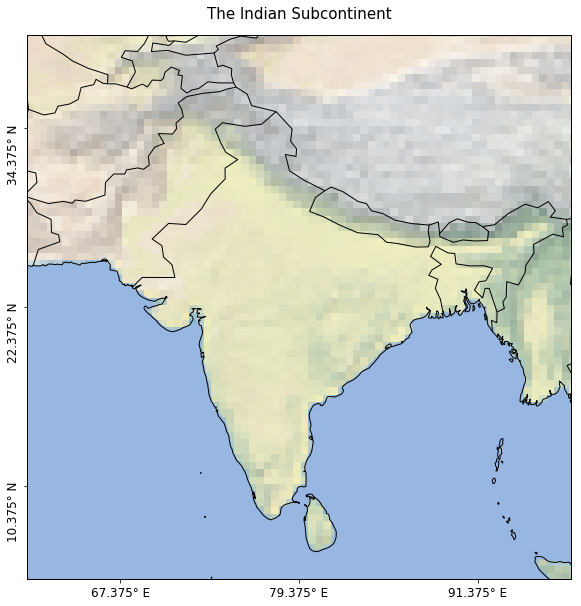
\includegraphics[width=0.5\linewidth]{./99_appendix/img/area_overview}
  \caption{The Indian subcontinent as extracted from TRMM.}
  \label{fig:trmm_area}
\end{figure}

The remainder of this work is then structured into two major parts that are both firmly connected to the behavior of the ISM. The first part (\cref{c:event_sync}) is dedicated to the analysis of extreme precipitation\footnote{Rainfall} events before, during and after the monsoon season. Such events are regularly seen all over India and represent one of the most significant challenges the local population faces from the ISM. Extreme rainfall can cause enormous damage by flooding cities or destruction of essential infrastructure. As such, there is a clear need to analyze and predict the spatial and temporal distribution of these extreme rainfall events.

Strongly basing our first part on the work of \citet{Stolbova.2015}, we extract extreme rainfall events from the TRMM precipitation dataset.

[TODO: short TRMM summary]

We then calculate the synchronicity of different pairs of locations\footnote{Simplified example: two locations are synchronous if an extreme event in one location tends to be followed by an extreme event in the other location.} and build a graph (a ``climate network'') connecting the most significantly synchronous locations.

Analysis of the resulting graph using graph centrality measures\footnote{Degree, Betweenness and PageRank} finally shows us the locations that are the most central and important in the graph. This knowledge could potentially help in the analysis or even prediction of monsoon behavior. For example, extreme rainfall in a location that is very central might be a reason to implement additional safety measures in connected locations.

The second major part of this work (\cref{c:part2}) deals with another critical issue regarding the Indian Summer Monsoon: the prediction of the onset date of monsoon. The onset date for a location in India depicts the point at which the monsoon reaches said location with strength and durability above a predefined threshold. We try to predict such an onset date for the Kerala region, which is generally one of the first locations reached by the ISM and as such marks the beginning of monsoon for the whole Indian subcontinent.

[TODO: short ERA-Interim summary]

For our onset prediction task, we build several neural network architectures using the Python Keras 2.0 and Tensorflow 1.4 libraries and describe the intuition of each. Experiments with each model allow us to evaluate and shortly summarize our most important findings. We iteratively improve upon the findings of each model, building models with vastly different architectures as well as for a number of datasets, features and combinations thereof (TRMM, ERA-Interim, different sets of onset dates). An overview and comparison of the learning capabilities of all models then serves as a conclusion to the second part.

Finally concluding our work in \cref{c:conclusion}, we summarize our overall findings and try to interpret the results of \cref{c:event_sync} and \cref{c:part2}. We additionally provide ideas for the improvement of our work and possible future research based on the topics of extreme event synchronization and monsoon onset prediction using neural networks.
